%%%%%%%%%%%%%%%%%%%%%%%%%%%%%%%%%%%%%%%%%%%%%%%%%%%%%%%%%%%%%%%%%%%%%%%%%%
%%LaTeX template for papers && theses									%%
%%Done by the incredible ||Z01db3rg||									%%
%%Under the do what ever you want license								%%
%%%%%%%%%%%%%%%%%%%%%%%%%%%%%%%%%%%%%%%%%%%%%%%%%%%%%%%%%%%%%%%%%%%%%%%%%% 

%start preamble
\documentclass[paper=a4,fontsize=11pt]{scrartcl}%kind of doc, font size, paper size
\usepackage[ngerman]{babel}%for special german letters etc			
%\usepackage{t1enc} obsolete, but some day we go back in time and could use this again
\usepackage[T1]{fontenc}%same as t1enc but better						
\usepackage[utf8]{inputenc}%utf-8 encoding, other systems could use others encoding
%\usepackage[latin9]{inputenc}			
\usepackage{amsmath}%get math done
\usepackage{amsthm}%get theorems and proofs done
\usepackage{graphicx}%get pictures & graphics done
\graphicspath{{pictures/}}%folder to stash all kind of pictures etc
\usepackage[pdftex,hidelinks]{hyperref}%for links to web
\usepackage{amssymb}%symbolics for math
\usepackage{amsfonts}%extra fonts
\usepackage []{natbib}%citation style
\usepackage{caption}%captions under everything
\usepackage{listings}
\usepackage[titletoc]{appendix}
\numberwithin{equation}{section} 
\usepackage[printonlyused,withpage]{acronym}%how to handle acronyms
\usepackage{float}%for garphics and how to let them floating around in the doc
\usepackage{cclicenses}%license!
\usepackage{xcolor}%nicer colors, here used for links
\usepackage{wrapfig}%making graphics floated by text and not done by minipage
\usepackage{dsfont}
\usepackage{stmaryrd}
\usepackage{geometry}
\usepackage{hyperref}
\usepackage{fancyhdr}
\usepackage{tabularx}
 \newcolumntype{L}{>{\raggedright\arraybackslash}X}

\pagestyle{fancy}
\lhead{Benjamin Tröster\\Netzwerke Seminaristische Übung (WS17/18)}
\rhead{FB 4 -- Angewandte Informatik\\ HTW-Berlin}
\lfoot{Übungsblatt 2 -- Bit-Arithmetik \& OSI-Layer I}
\cfoot{}
\fancyfoot[R]{\thepage}
\renewcommand{\headrulewidth}{0.4pt}
\renewcommand{\footrulewidth}{0.4pt}

\lstdefinestyle{Bash}{
  language=bash,
  showstringspaces=false,
  basicstyle=\small\sffamily,
  numbers=left,
  numberstyle=\tiny,
  numbersep=5pt,
  frame=trlb,
  columns=fullflexible,
  backgroundcolor=\color{gray!20},
  linewidth=0.9\linewidth,
  %xleftmargin=0.5\linewidth
}


\newlength\labelwd
\settowidth\labelwd{\bfseries viii.)}
\usepackage{tasks}
\settasks{counter-format =tsk[a].), label-format=\bfseries, label-offset=3em, label-align=right, label-width
=\labelwd, before-skip =\smallskipamount, after-item-skip=0pt}
\usepackage[inline]{enumitem}
\setlist[enumerate]{% (
labelindent = 0pt, leftmargin=*, itemsep=12pt, label={\textbf{\arabic*.)}}}

\pdfpkresolution=2400%higher resolution

%settings colors for links
\hypersetup{
    colorlinks,
    linkcolor={blue!50!black},
    citecolor={blue},
    urlcolor={blue!80!black}
}

%\usepackage[pagetracker=true]{biblatex}

%%here begins the actual document%%
\newcommand{\horrule}[1]{\rule{\linewidth}{#1}} % Create horizontal rule command with 1 argument of height


\DeclareMathOperator{\id}{id}

\title{	
\normalfont \normalsize 
\textsc{Übungsblatt 1 -- Shell Grundlagen}
}

\begin{document}
\center
\Large{\textbf{Übungsblatt 2 -- Bit-Arithmetik \& OSI-Layer I}}\\
\large{\textbf{\textcolor{red}{Hinweis:} Versuchen Sie die Übungsblätter soweit wie möglich ohne Hilfe von Google, Stackoverflow, Stackexchange zu lösen. Sie sollen eigene Lösungswege finden und nicht professionell Suchmaschinen bedien können. Ausnahmen sind natürlich Aufgaben, in denen explizit recherchiert werden soll}
\begin{center}\Large{\textbf{Bit-Arithmetik}}\end{center}\vskip0.25in
%\setlist[enumerate, 1]{itemsep=\baselineskip}
\begin{enumerate}
\item Wandeln Sie die Dezimalzahlen der Tabelle in die gegebenen Zahlensysteme um.
\begin{table}[H]	
\begin{tabular}{|c|c|c|c|c|}
  \hline
 Dezimal & 13107 & 6872 & -733 & 65536 \\ \hline 
  Binär & & & &  \\ \hline
  Oktal & & & &  \\ \hline
  Hexadezimal & & & &  \\ \hline
  Zur Basis 13 & & & & \\ \hline
\end{tabular}
\end{table}
	\item Was ist der Unterschied zwischen 1 kb, 1 kB und 1 KiB?
	\item Verbreitete Annahmen zu Daten sind:
	\begin{itemize}
		\item Daten sind heute einfach zu speichern.
		\item Daten sind heute einfach zu transportieren bzw. zu übertragen.
	\end{itemize}
	In diese Übung untersuchen Sie, ob die Aussagen korrekt sind.
	\begin{tasks}(1)
		\task Das SKA (\href{https://skatelescope.org/}{Square Kilometer Array}) wird in seiner ersten Phase sehr große Datenmengen erzeugen. Voraussichtlich werden im ersten Jahr etwa 300 PB anfallen. Welche Höhe würden bei diesen Datenmengen erreicht werden? Wie hoch wäre ein Stapel, wenn zur Speicherung ...
		\begin{itemize}
		\item CDs (Kapazität: 600 MB, Dicke: 1,2 mm) verwendet würden?
		\item DVDs (Kapazität: 4,3 GB, Dicke: 1,2 mm) verwendet werden?
		\item Blu-Ray-Disks (Kapazität: 25 GB, Dicke: 1,2 mm) verwendet werden?
		\item Festplatten (Kapazität: 2 TB, Dicke: 2,5 cm) verwendet werden?
		\end{itemize}	 
	\end{tasks}
	
\end{enumerate}

\begin{center}\Large{\textbf{Bandbreitenberechnung}}\end{center}\vskip0.25in
%\setlist[enumerate, 1]{itemsep=\baselineskip}

\begin{enumerate}
\begin{minipage}{0.7\textwidth}
\item Der preußische optische Telegraf (1832-1849) war ein telegrafisches Kommunikationssystem zwischen Berlin und Koblenz in der Rheinprovinz.\\
Behördliche und militärische Nachrichten konnten mittels optischer Signale über eine Distanz von fast 550 km via 62 Telegrafenstationen übermitteln werden.\\
Jede Station verfügte über 6 Telegrafenarme mit je 4 Positionen zur Kodierung.
\begin{tasks}(1)
	\task~ Datentransferrate: Wie viele Bits können pro Sekunde übertragen werden, wenn man alle 10 Sekunden eine neue Einstellung der Telegrafenarme vornehmen kann?
	\task~ Latenz: Wie groß ist die Ende-zu-EndeVerzögerung, wenn jede Station 1 Minute für die Weiterleitung benötigt? Einfacher gefragt: Wie lange dauert die Übertragung einer Nachricht von Berlin nach Koblenz?
\end{tasks}
\end{minipage}%
\begin{minipage}{0.3\textwidth}
\begin{figure}[H]
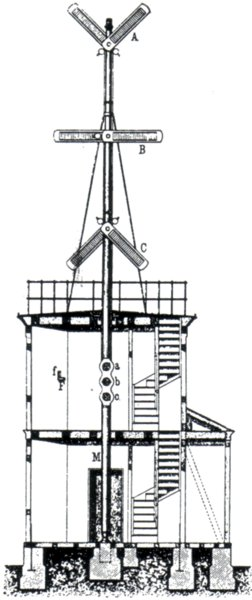
\includegraphics[scale=0.5]{telegraph}
\end{figure}
\end{minipage} \hfill

\item Eine Taube kann eine Geschwindigkeit von 100 km/h erreichen und dabei einen USB-Stick mit einer Kapazität von bis 512 GByte tragen. Bis zu welcher Reichweite hat die Taube die höhere Datenrate gegenüber einer 1 GBit-Leitung? Angenommen die Taube könnte unendlich lange die Maximalgeschwindigkeit halten.
\end{enumerate}

\begin{center}\Large{\textbf{Topologien \& Geräte}}\end{center}\vskip0.25in
%\setlist[enumerate, 1]{itemsep=\baselineskip}
\begin{enumerate}
\item Was definiert den \glqq physical layer\grqq\ im OSI-Modell? Was ist die Aufgabe des \glqq physical layers\grqq?
\item Was beschreibt die physische Topologie eines Computernetzwerks?
\item  Was beschreibt die logische Topologie eines Computernetzwerks?
\item Es existieren unterschiedliche Netzwerktopologien (Bus, Ring, Maschen,
Baum und Zelle). Fügen Sie in die folgende Tabelle die Namen der Netzwerktopologien
ein, auf die die gegebenen Aussagen in der Tabelle zutreffen.
\begin{table}[H]
\begin{tabularx}{\linewidth}{|L|c|} \hline
 Aussage & Topologie(n) \\ \hline
 Ein Kabelausfall kann das Netzwerk in zwei funktionsfähige Teile unterteilen & \\ \hline
 Diese Topologie enthält einen Single Point of Failure \newline
 (Ein Single Point of Failure kann ein Gerät oder ein Kabel sein) & \\ \hline
 Diese Topologie enthält einen Performance-Flaschenhals  & \\ \hline
 WLAN ohne Access Point verwendet diese Topologie & \\ \hline
 Diese Topologie verwendet Token Ring (logisch) & \\ \hline
 Ein Kabelausfall führt zum kompletten Netzwerkausfall & \\ \hline
 Diese Topologie enthält keine zentrale Komponente & \\ \hline
 WLAN mit Access Point verwendet diese Topologie & \\ \hline
 Moderne Ethernet-Standards verwenden diese Topologie & \\ \hline
\end{tabularx}
\end{table}
\item Nenne Sie Beispiele für Übertagungsmedien. Wird für die Kommunikation immer ein Übertragungsmedium benötigt?
\item Auf Netzwerkkabeln befinden sich Zeichenfolgen mit Buchstaben, Zahlen und Sonderzeichen. Deren Inhalt ist auf den ersten Blick schwer zu verstehen.\\
Beispielsweise:\\
\texttt{E188601 (UL) TYPE CM $75^\circ$C LL84201 CSA TYPE CMG FT4 CAT.5E PATCH CABLE
TO TIA/EIA 568A STP 26AWG STRANDED}
Recherchieren Sie dazu folgende Fragen:
\begin{tasks}(1)
	\task Was bedeutet STRANDED?
	\task Existieren auch Kabel, die nicht STRANDED sind?
	\task Was bedeutet PATCH?
	\task Existieren auch Kabel, die nicht PATCH sind?
	\task Was ist der Unterschied zwischen PATCH-Kabeln und anderen Kabeln?
	\task Was bedeutet die Information 24 AWG oder 26AWG?
	\task Was bedeutet die Information UL CM FT1/FT4 zusammen mit einer Gradangabe
(z.B. $60^\circ$ oder $75^\circ$C)?
\end{tasks}
\end{enumerate}
\end{document}